\section{Sloan actuator structure} \label{circles}

As said in Section \ref{reminder}, the Sloan telescope arrangement is made of 500 actuators, in an hexagonal shape. In the MOONS project, actuators types and position were listed in a cfg file. For time and practical reasons, this has been changed. A program called "circles.py" has been created to contain all actuators position and properties. The program is launched at each software's run, ensuring that, if a structure's parameter is changed (space between two parameters, fiber properties of several actuators etc.), the program will be automatically updated.

\begin{figure}[h]
\begin{center}
	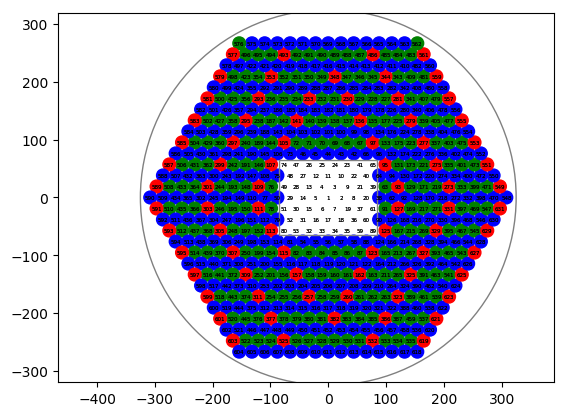
\includegraphics[width=\textwidth]{circles/sloan_arrangement.png}
	\caption{Actuators structure for the Sloan project.}
	\label{fig:sloan:arrangement}
\end{center}
\end{figure}

The script creates the structure shown on Figure \ref{fig:sloan:arrangement}. One can compare it with the structure desired shown on Figure \ref{fig:reminder:sloan_arrangement}. The creation and indexation of actuators work as follow :

\begin{enumerate}
	\item A first actuator is created on position (0, 0).
	\item Then, using several functions available in the Appendix 1, a layer made of 6 actuators is created, beginning by the one on the right of the first actuator (actuator 2). The second function creates an actuator (actuator 3) on the top left of the preceding actuator, the third function creates an actuator (actuator 4) on the left of actuator 3 and so on. As the first layer is made of 6 actuators, each function is applied once.
	\item The second layer, made of 12 actuators, is made by applying the first function to create actuator 8. Then the second function is applied two times, creating actuators 9 and 10, and so on until the layer is finished.
	\item The rest of the structure is made by applying Step 3 until a certain quantity of actuator has been created.
\end{enumerate} 

The indexation and construction of the structure is illustrated in the Appendix 1.
\\

 Then, the second part of the program classifies each actuator in one of the four following categories: empty, fiducial, IR or visible. Each actuator positioned in the rectangle in the middle of the telescope is set in the Empty category. Each actuator positioned on a fiducial slot as shown on Figure \ref{fig:sloan:arrangement} is set in the Fiducial category. As shown on Figure \ref{fig:sloan:arrangement}, every actuator containing an IR fibre have similar y-coordinates, which is a certain real number times any discrete (positive, negative or null) number; any actuator which is not an Empty or a Fiducial having the aforementioned y-coordinate property is set as IR. Any other actuator, plus the two actuators on the top left and top right of the arrangement (see Figure \ref{fig:sloan:arrangement}) are set as Visible.
\\

The script works for the structure set on December 2017. It is still possible to modify it easily; for instance :

\begin{itemize}
	\item If the middle rectangle size is increased (or decreased), the only update to make is the addition (or subtraction) of actuator's indexes in the text file "empty.txt".
	\item If some actuators will be replaced by fiducial (or some fiducial removed), the only update is the addition (or subtraction) of actuator's indexes in the text file "fiducial.txt".
	\item If the dimensions of the structure are changed (space between actuators), the program updates automatically the list of actuators set as IR.
	\item If new actuators have to be added on the limits of the existing ones to approach the circular shape, only two steps are required: adding new actuator layers, and adding a new requirement such as the radial coordinate of the actuator has to be inferior to the radius of the telescope (or manually classifying the actuators created outside of the focal plane as Empty).
\end{itemize}

An example of each one of those adjustment is shown on Figure \ref{fig:sloan:examples}.

\begin{figure}[h]
	\begin{center}
		\begin{subfigure}{0.85\textwidth}
			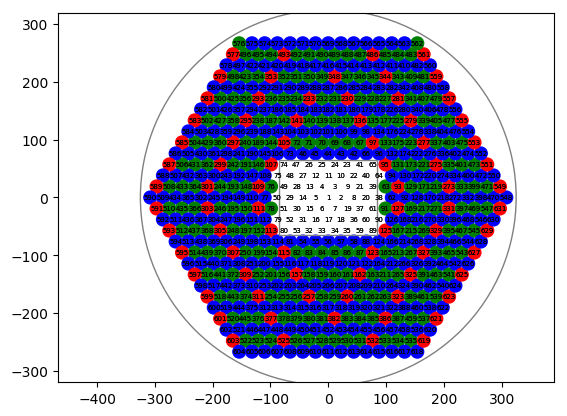
\includegraphics[width=\textwidth]{circles/sloan_adding_empty.png}
			\caption{}
		\end{subfigure}

		\begin{subfigure}{0.85\textwidth}
			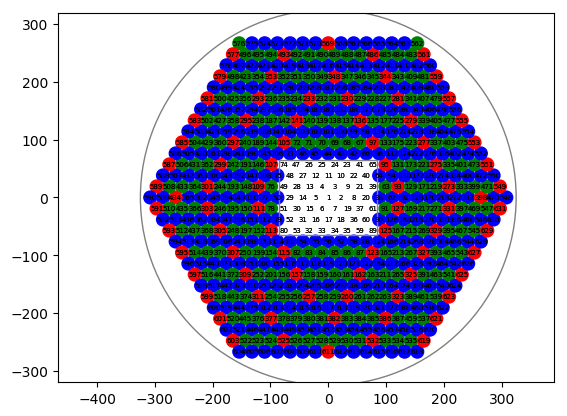
\includegraphics[width=\textwidth]{circles/sloan_adding_fiducial.png}
			\caption{}
		\end{subfigure}
	\end{center}
\end{figure}
		
\begin{figure}[h]\ContinuedFloat
\begin{center}
		\begin{subfigure}{0.85\textwidth}
			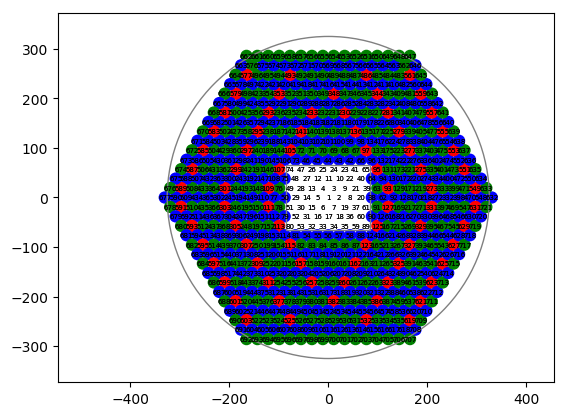
\includegraphics[width=\textwidth]{circles/sloan_adding_layer.png}
			\caption{}
		\end{subfigure}
		
		\begin{subfigure}{0.85\textwidth}
			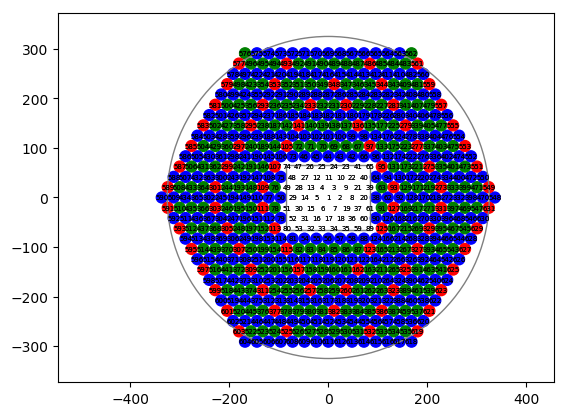
\includegraphics[width=\textwidth]{circles/sloan_adding_separation.png}
			\caption{}
		\end{subfigure}
		\caption{Examples of adjustments made on the actuator's structure only by modifying text files. (a) Addition of six indexes (38, 50, 64, 75, 79, 90) in the file empty.txt. (b) Addition of four indexes (398, 434, 569, 611) in the file fiducial.txt. (c) Addition of a layer by modifying an entry in the file parameters.txt. (d) Increase of the separation length between actuators by modifying an entry in the file parameters.txt.}
		\label{fig:sloan:examples}
	\end{center}
\end{figure}